\documentclass[aspectratio=169,11pt]{beamer}

\usetheme{Madrid}
\usecolortheme{default}
\setbeamertemplate{navigation symbols}{}
\setbeamertemplate{footline}[frame number]

\usepackage[T1]{fontenc}
\usepackage{lmodern}
\usepackage{amsmath,amssymb}
\usepackage{graphicx}
\usepackage{tikz}
\usetikzlibrary{arrows.meta,positioning,fit,shapes.misc}

\definecolor{rugblue}{RGB}{0,74,153}
\definecolor{softblue}{RGB}{229,239,252}
\definecolor{softgreen}{RGB}{229,246,236}
\definecolor{softorange}{RGB}{255,241,224}
\definecolor{softgray}{RGB}{245,245,245}
\definecolor{darkgray}{RGB}{70,70,70}

\setbeamercolor{structure}{fg=rugblue}
\setbeamercolor{frametitle}{fg=white,bg=rugblue}
\setbeamercolor{title}{fg=white,bg=rugblue}
\setbeamercolor{block title}{fg=white,bg=rugblue}
\setbeamercolor{block body}{bg=softgray}

\newcommand{\coursepath}{..}
\newcommand{\lecturefig}[1]{\coursepath/Lectures/#1}
\newcommand{\presentationfig}[1]{\coursepath/PresentationFigures/#1}

\tikzset{
  box/.style={
    rounded corners=2pt,
    draw=rugblue,
    very thick,
    align=center,
    inner sep=5pt,
    fill=softblue,
    font=\small
  },
  greenbox/.style={box, fill=softgreen, draw=green!45!black},
  orangebox/.style={box, fill=softorange, draw=orange!65!black},
  graybox/.style={box, fill=softgray, draw=darkgray},
  arrow/.style={-{Latex[length=2.2mm]}, thick, draw=darkgray}
}

\title[Interactive Statistics Course]{Developing a Reproducible, Interactive Statistics Course}
\subtitle{Jupyter notebooks, Git, Colab, VS Code, Overleaf, HPC, and AI-supported course maintenance}
\author{Daan Meerburg}
\institute{University of Groningen}
\date{Academic Staff Presentation}

\begin{document}

\begin{frame}
  \titlepage
\end{frame}

\begin{frame}{What I Built}
  \begin{columns}[T,totalwidth=\textwidth]
    \begin{column}{0.52\textwidth}
      \begin{itemize}
        \item New statistics course for third-year BSc Physics students
        \item 12 Jupyter lecture notebooks
        \item Colab to execute in the cloud
        \item Alt: VS Code/Git route for durable local editing
        \item Board notes, quizzes, assignments, projects, exams, rubrics
        \item Development workflow on the HPC, synchronized with Git and Overleaf
      \end{itemize}
    \end{column}
    \begin{column}{0.44\textwidth}
      \begin{block}{Central format}
        \Large Jupyter notebooks
      \end{block}
      \begin{block}{Notebook contents}
        text, equations, code, figures, exercises
      \end{block}
      \begin{block}{Student access}
        Colab or local VS Code/Git
      \end{block}
    \end{column}
  \end{columns}
\end{frame}

\begin{frame}{Course Design}
  \begin{columns}[T,totalwidth=\textwidth]
    \begin{column}{0.52\textwidth}
      \begin{block}{Keep these together}
        \begin{itemize}
          \item Theory and Math
          \item Python implementation
          \item Plots and numerical output
          \item Execution and interpretation
        \end{itemize}
      \end{block}
      \vspace{0.25cm}
      Students can move between formulas, code, and interpretation in the same environment.
    \end{column}
    \begin{column}{0.44\textwidth}
      \begin{block}{Why notebooks}
        A Jupyter notebook puts explanation, code cells, output, and short checks in one document.
      \end{block}
      \begin{block}{In class}
        Students can rerun an example while the statistical idea is being discussed.
      \end{block}
    \end{column}
  \end{columns}
\end{frame}

\begin{frame}{Design Principle: One Executable Document}
  \begin{columns}[T,totalwidth=\textwidth]
    \begin{column}{0.5\textwidth}
      Each lecture notebook combines:
      \begin{itemize}
        \item Text and equations
        \item Python code
        \item Figures and simulations
        \item Short exercises and larger assignments
        \item Links to data and external resources
      \end{itemize}
      \vspace{0.2cm}
      The lecture note is also the file students run and edit.
    \end{column}
    \begin{column}{0.47\textwidth}
      \begin{block}{Notebook as lecture note}
        explanation, notation, examples
      \end{block}
      \begin{block}{Notebook as executable file}
        runnable code, plots, data
      \end{block}
      \begin{block}{Notebook as exercise space}
        change assumptions and rerun
      \end{block}
    \end{column}
  \end{columns}
\end{frame}

\begin{frame}{Two Student Routes}
  \begin{columns}[T,totalwidth=\textwidth]
    \begin{column}{0.48\textwidth}
      \begin{block}{Route 1: Colab}
        \begin{itemize}
          \item click the Colab badge
          \item run cells immediately
          \item many common Python libraries already available
          \item use Drive/download/GitHub export for lasting copies
        \end{itemize}
      \end{block}
    \end{column}
    \begin{column}{0.48\textwidth}
      \begin{block}{Route 2: VS Code + Git}
        \begin{itemize}
          \item Fork or clone the repository
          \item Edit notebooks locally
          \item Commit and maintain a personal version
          \item More package setup, more flexibility
        \end{itemize}
      \end{block}
    \end{column}
  \end{columns}
  \vspace{0.35cm}
  \begin{block}{Trade-off}
    Colab is easiest for class use, but runtime state is temporary. VS Code and Git require local setup, but give students a persistent fork they can edit and maintain.
  \end{block}
\end{frame}

\begin{frame}{Course Arc}
  \begin{columns}[T,totalwidth=\textwidth]
    \begin{column}{0.31\textwidth}
      \begin{block}{Lectures 1--4}
        \begin{itemize}
          \item Introduction
          \item Probability
          \item Distributions
          \item Correlations
        \end{itemize}
      \end{block}
    \end{column}
    \begin{column}{0.31\textwidth}
      \begin{block}{Lectures 5--7}
        \begin{itemize}
          \item Likelihood functions
          \item Maximum likelihood estimation (MLE)
          \item Bootstrap and jackknife
          \item Outliers and model comparison
        \end{itemize}
      \end{block}
    \end{column}
    \begin{column}{0.31\textwidth}
      \begin{block}{Lectures 8--12}
        \begin{itemize}
          \item Priors and posteriors
          \item Maximum a posteriori (MAP) estimation
          \item Marginalization
          \item Gibbs sampling
          \item MCMC and nested sampling
        \end{itemize}
      \end{block}
    \end{column}
  \end{columns}
  \vspace{0.35cm}
  \centering
  \large foundations $\rightarrow$ frequentist inference $\rightarrow$ Bayesian inference
\end{frame}

\begin{frame}{Example Visuals from the Course}
  \begin{columns}[T,totalwidth=\textwidth]
    \begin{column}{0.56\textwidth}
      \centering
      \includegraphics[width=\linewidth,height=0.64\textheight,keepaspectratio]{\lecturefig{CosmicRaysFlux.png}}
      \vspace{0.15cm}

      \small Data, uncertainty, and scaling laws appear directly in the notebook.
    \end{column}
    \begin{column}{0.4\textwidth}
      \begin{block}{Teaching use}
        \begin{itemize}
          \item Students run the same examples
          \item Plots are tied to code
          \item Assumptions can be changed
          \item Interpretation follows directly
          \item Student can run and modify the notebook in their own time 
        \end{itemize}
      \end{block}
    \end{column}
  \end{columns}
\end{frame}

\begin{frame}{Why use HPC for Development?}
  \begin{columns}[T,totalwidth=\textwidth]
    \begin{column}{0.48\textwidth}
      My development workspace is centered on the HPC:
      \begin{itemize}
        \item Accessible from all machines
        \item Course repository cloned and version controlled
        \item Overleaf projects linked through Git
        \item Notebooks, notes, assignments, exams, and rubrics in one workflow
        \item Easy to maintain and update the course for future years 
      \end{itemize}
    \end{column}
    \begin{column}{0.5\textwidth}
      \centering
      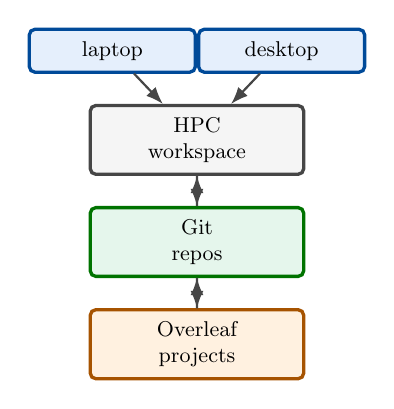
\begin{tikzpicture}[node distance=0.45cm, scale=0.86, transform shape]
        \node[graybox, text width=2.8cm] (hpc) {HPC\\workspace};
        \node[box, above=of hpc, xshift=-1.25cm, text width=2.1cm] (laptop) {laptop};
        \node[box, above=of hpc, xshift=1.25cm, text width=2.1cm] (desktop) {desktop};
        \node[greenbox, below=of hpc, text width=2.8cm] (git) {Git\\repos};
        \node[orangebox, below=of git, text width=2.8cm] (overleaf) {Overleaf\\projects};
        \draw[arrow] (laptop) -- (hpc);
        \draw[arrow] (desktop) -- (hpc);
        \draw[arrow] (hpc) -- (git);
        \draw[arrow] (git) -- (hpc);
        \draw[arrow] (git) -- (overleaf);
        \draw[arrow] (overleaf) -- (git);
      \end{tikzpicture}
    \end{column}
  \end{columns}
\end{frame}

\begin{frame}{Why Try AI in This Course?}
  \begin{columns}[T,totalwidth=\textwidth]
    \begin{column}{0.69\textwidth}
      \centering
      \includegraphics[width=\linewidth,height=0.64\textheight,keepaspectratio]{\presentationfig{tpbench_flagship_2026.png}}
    \end{column}
    \begin{column}{0.28\textwidth}
      \footnotesize
      \begin{block}{TPBench}
        Theoretical-physics problems from undergraduate to research level.
      \end{block}
      \begin{block}{Takeaway}
        GPT-5.5 is among the strongest models, with performance even on research-level problems. BSc problems are no almost 100\% solved. 
      \end{block}
      \vspace{0.05cm}
      {\tiny Source: TPBench, May 2026.}
    \end{column}
  \end{columns}
\end{frame}

\begin{frame}{Scientific Coding Agents Are Being Benchmarked}
  \begin{columns}[T,totalwidth=\textwidth]
    \begin{column}{0.69\textwidth}
      \centering
      \includegraphics[
        page=7,
        width=\linewidth,
        height=0.62\textheight,
        keepaspectratio,
        trim=1.35in 8.55in 1.00in 0.95in,
        clip
      ]{\presentationfig{colliderbench.pdf}}
    \end{column}
    \begin{column}{0.28\textwidth}
      \footnotesize
      \begin{block}{Collider-Bench}
        Agents reproduce LHC analyses using public papers and open software.
      \end{block}
      \begin{block}{Takeaway}
        GPT-5.5 is competitive, but the paper still finds a gap to physicist-in-the-loop workflows.
      \end{block}
      \vspace{0.1cm}
      {\tiny Source: Faroughy et al., arXiv:2605.13950, Fig. 2.}
    \end{column}
  \end{columns}
\end{frame}

\begin{frame}{Where AI Fit}
  \begin{columns}[T,totalwidth=\textwidth]
    \begin{column}{0.54\textwidth}
      I used AI for specific course-development tasks:
      \begin{itemize}
        \item Revise notebook explanations
        \item Turn notebook material into board-style notes
        \item Draft assignments, projects, exams, and rubrics
        \item Check consistency across course components
        \item Maintain repositories: diffs, commits, pushes, public/private separation
        \item List is growing as new AI tools become available and improve 
      \end{itemize}
    \end{column}
    \begin{column}{0.43\textwidth}
      \centering
      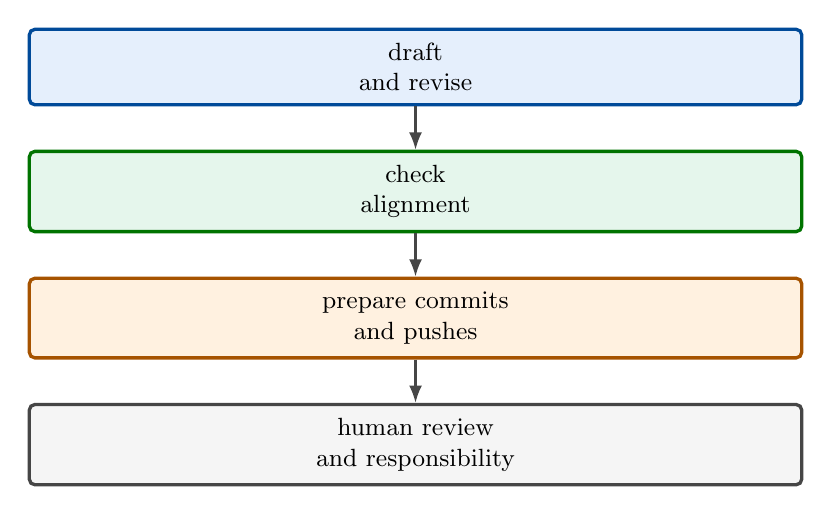
\begin{tikzpicture}[node distance=0.55cm]
        \node[box, text width=0.78\linewidth] (draft) {draft\\and revise};
        \node[greenbox, below=of draft, text width=0.78\linewidth] (check) {check\\alignment};
        \node[orangebox, below=of check, text width=0.78\linewidth] (git) {prepare commits\\and pushes};
        \node[graybox, below=of git, text width=0.78\linewidth] (human) {human review\\and responsibility};
        \draw[arrow] (draft) -- (check);
        \draw[arrow] (check) -- (git);
        \draw[arrow] (git) -- (human);
      \end{tikzpicture}
    \end{column}
  \end{columns}
\end{frame}

\begin{frame}{From Lecture to Assessment}
  \centering
  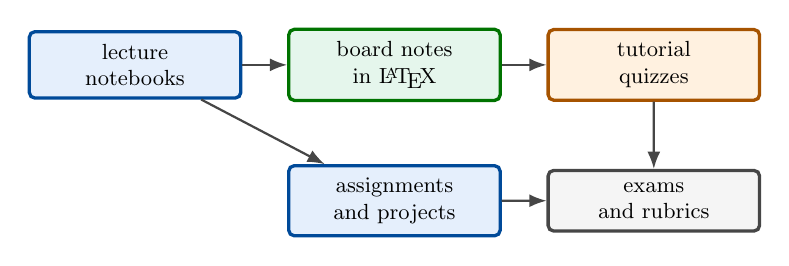
\begin{tikzpicture}[node distance=0.65cm, scale=0.88, transform shape]
    \node[box, text width=2.7cm] (lecture) {lecture\\notebooks};
    \node[greenbox, right=of lecture, text width=2.7cm] (board) {board notes\\in \LaTeX};
    \node[orangebox, right=of board, text width=2.7cm] (quiz) {tutorial\\quizzes};
    \node[box, below=0.9cm of board, text width=2.7cm] (assign) {assignments\\and projects};
    \node[graybox, right=of assign, text width=2.7cm] (exam) {exams\\and rubrics};
    \draw[arrow] (lecture) -- (board);
    \draw[arrow] (board) -- (quiz);
    \draw[arrow] (lecture) -- (assign);
    \draw[arrow] (assign) -- (exam);
    \draw[arrow] (quiz) -- (exam);
  \end{tikzpicture}
  \vspace{0.6cm}

  \begin{block}{Design goal}
    Keep explanation, practice, project work, and assessment aligned.
  \end{block}
\end{frame}

\begin{frame}{AI-Supported Repository Workflow}
  \centering
  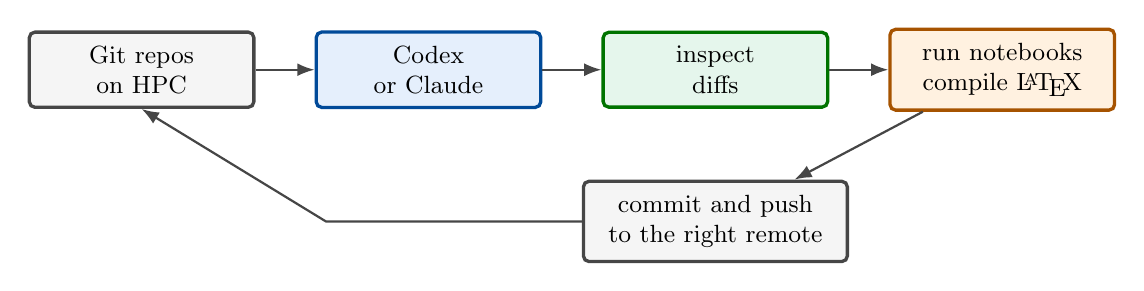
\begin{tikzpicture}[node distance=0.75cm]
    \node[graybox, text width=2.5cm] (repo) {Git repos\\on HPC};
    \node[box, right=of repo, text width=2.5cm] (ai) {Codex\\or Claude};
    \node[greenbox, right=of ai, text width=2.5cm] (diff) {inspect\\diffs};
    \node[orangebox, right=of diff, text width=2.5cm] (test) {run notebooks\\compile \LaTeX};
    \node[graybox, below=0.9cm of diff, text width=3.0cm] (push) {commit and push\\to the right remote};
    \draw[arrow] (repo) -- (ai);
    \draw[arrow] (ai) -- (diff);
    \draw[arrow] (diff) -- (test);
    \draw[arrow] (test) -- (push);
    \draw[arrow] (push.west) -- ++(-3.25,0) -- (repo.south);
  \end{tikzpicture}
  \vspace{0.6cm}

  \begin{block}{Control point}
    The useful part is not automation by itself. The useful part is that changes are visible as diffs, notebooks can be rerun, \LaTeX{} can be compiled, and I decide what is released.
  \end{block}
\end{frame}

\begin{frame}{Inference Examples in Notebooks}
  \begin{columns}[T,totalwidth=\textwidth]
    \begin{column}{0.49\textwidth}
      \centering
      \includegraphics[height=0.64\textheight]{\lecturefig{Gibbs.png}}
      \vspace{0.1cm}

      \small Gibbs sampling
    \end{column}
    \begin{column}{0.49\textwidth}
      \centering
      \includegraphics[height=0.64\textheight]{\lecturefig{Dynesty_Sampler.png}}
      \vspace{0.1cm}

      \small Nested sampling
    \end{column}
  \end{columns}
\end{frame}

\begin{frame}{Benefits for Teaching}
  \begin{columns}[T,totalwidth=\textwidth]
    \begin{column}{0.52\textwidth}
      \begin{itemize}
        \item Students can rerun computational examples.
        \item Exercises become closer to real research practice.
        \item Lectures, assignments, projects, and exams stay aligned.
        \item Updates are easier because the course is version controlled.
        \item Colleagues can inspect, reuse, or adapt parts of the course.
      \end{itemize}
    \end{column}
    \begin{column}{0.44\textwidth}
      \centering
      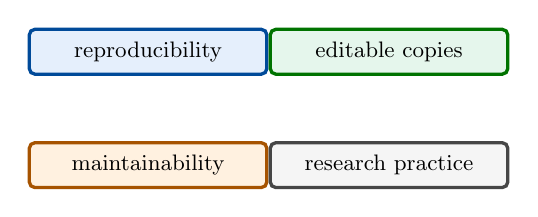
\begin{tikzpicture}[scale=0.9, transform shape]
        \node[box, text width=3.0cm] at (0,1.4) {reproducibility};
        \node[greenbox, text width=3.0cm] at (3.4,1.4) {editable copies};
        \node[orangebox, text width=3.0cm] at (0,-0.2) {maintainability};
        \node[graybox, text width=3.0cm] at (3.4,-0.2) {research practice};
      \end{tikzpicture}
    \end{column}
  \end{columns}
\end{frame}

\begin{frame}{Things to keep in mind}
  \begin{columns}[T,totalwidth=\textwidth]
    \begin{column}{0.49\textwidth}
      \begin{block}{Challenges}
        \begin{itemize}
          \item Colab sessions are convenient but temporary.
          \item VS Code/Git gives flexibility, but needs setup.
          \item Notebooks can hide complexity.
          \item AI can produce plausible errors.
        \end{itemize}
      \end{block}
    \end{column}
    \begin{column}{0.49\textwidth}
      \begin{block}{Mitigations}
        \begin{itemize}
          \item Explicit persistence/forking instructions (lecture 1)
          \item During lecture I combine blackboard presentation with live notebook execution
          \item Students are encouraged to read and understand the code, not just run it
          \item AI is used as a drafting tool, but all changes are reviewed before release
          \item Private repos for exams and solutions, public repos for lectures and assignments
        \end{itemize}
      \end{block}
    \end{column}
  \end{columns}
\end{frame}

\begin{frame}{Take-Home Message}
  \begin{center}
    \Large
    The course is built around version-controlled Jupyter notebooks. It uses many modern tools to make the material interactive, reproducible, and maintainable. AI is a helpful assistant, but human review and control are essential.
  \end{center}
  \vspace{0.4cm}
  \begin{itemize}
    \item Students can read, run, fork, and modify the lectures.
    \item They can choose Colab for access or VS Code/Git for persistence.
    \item Git, Overleaf, and the HPC make the material easier to maintain.
    \item AI helps with drafting and repository maintenance, but changes are reviewed before release.
  \end{itemize}
\end{frame}

% \begin{frame}{Possible Live Demo}
%   \begin{enumerate}
%     \item Open the GitHub repository README.
%     \item Click the Colab badge.
%     \item Run one short simulation cell.
%     \item Change one parameter and rerun.
%     \item Briefly show the alternative: a local VS Code/Git checkout.
%   \end{enumerate}
%   \vspace{0.5cm}
%   Good candidate notebooks:
%   \begin{itemize}
%     \item \texttt{Lecture\_03\_PDM.ipynb}: distributions and confidence levels
%     \item \texttt{Lecture\_06\_PDM.ipynb}: outliers, model comparison, bootstrap
%     \item \texttt{Lecture\_10\_PDM.ipynb}: Monte Carlo and MCMC
%   \end{itemize}
% \end{frame}

\end{document}
